\chapter{Planning and Architecture}
\section*{Introduction}
\addcontentsline{toc}{section}{Introduction}
This chapter turns the product vision of \projectname{} into the requirements, diagrams, backlog, sprint plan, and architecture used to guide implementation. The platform covers partnership requests, employee operations, partner self-service, business intelligence, document handling, scoring, and AI-assisted decision support.
\section{Requirements Analysis and Specification}
The requirements analysis defines who uses the platform and what each surface must provide. It separates functional needs from quality constraints so the later architecture can trace every major choice back to a concrete requirement.
\subsection{Actor Identification}
The platform distinguishes six main actors. Five are internal employee roles with access to the employee portal, while Partner represents external organizations using the self-service portal.

\begin{table}[H]
  \centering
  \caption{Actor identification for \projectname{}}
  \begin{tabularx}{\textwidth}{>{\bfseries\raggedright\arraybackslash}p{2.7cm}>{\raggedright\arraybackslash}p{3.3cm}X}
    \toprule
    Actor & Scope & Main responsibilities \\
    \midrule
    Admin & Global platform governance & Manages employee accounts, access rules, audit traces, reference data, and consistency. \\
    Manager & Partnership supervision & Reviews partner portfolios, tracks partnerships, validates lifecycle decisions, monitors project health, and uses AI-assisted insights. \\
    Commercial & Business relationship operations & Manages partner contacts, offers, meetings, communications, opportunities, and follow-up for customer, supplier, marketing, and university partnerships. \\
    Analyst & Reporting and intelligence & Explores dashboards, indicators, partner scores, churn signals, document evidence, and warehouse views. \\
    HR & Academic and workforce workflows & Handles roster views, university collaboration workflows, student recruitment records, conversion indicators, and HR partnership events. \\
    Partner & External self-service access & Uses its dashboard, profile, offers, events, contacts, documents, notifications, statistics, and collaboration areas. \\
    \bottomrule
  \end{tabularx}
\end{table}
\subsection{Functional Requirements}
The functional requirements cover the public surface, employee portal, partner portal, business intelligence, and AI assistant.

\begin{table}[H]
  \centering
  \caption{Functional requirements}
  \begin{tabularx}{\textwidth}{>{\bfseries\raggedright\arraybackslash}p{1.2cm}>{\raggedright\arraybackslash}p{3.4cm}X}
    \toprule
    ID & Area & Requirement \\
    \midrule
    FR1 & Access and identity & Authenticate employees and partners, recover the server session, and route each role to its workspace. \\
    FR2 & Public partnership entry & Present the partnership value proposition and let external organizations submit structured partnership requests. \\
    FR3 & Partner lifecycle & Create, update, categorize, score, negotiate, suspend, and track partners through a controlled lifecycle with status history. \\
    FR4 & Relationship communications & Manage contacts, meetings, events, notifications, and communication records linked to partners. \\
    FR5 & Documents and offers & Upload, organize, retrieve, and expose partner documents and offers according to ownership and role permissions. \\
    FR6 & Partner self-service & Provide external partners with a restricted portal for profile data, offers, events, documents, notifications, contacts, statistics, and collaboration flows. \\
    FR7 & Projects and delivery & Track projects, milestones, tasks, team allocation, progress, budget indicators, project documents, and delivery health. \\
    FR8 & Business intelligence & Display analytical dashboards backed by a dedicated data warehouse, including portfolio, category, project, and partner-performance metrics. \\
    FR9 & Agentic AI assistant & Provide a streamed AI workspace that can call validated tools for partner search, analytics, scoring, recommendations, project health analysis, report generation, and document retrieval. \\
    FR10 & Report generation & Generate, preview, edit, and export executive reports built from real platform data and AI-assisted synthesis. \\
    FR11 & Governance and audit & Record significant actions, status changes, communication events, AI tool traces, generated reports, and security-relevant access events. \\
    FR12 & Configuration and maintainability & Keep reusable UI primitives, server services, database access, AI tools, and authentication utilities separated by responsibility. \\
    \bottomrule
  \end{tabularx}
\end{table}
\subsection{Non-Functional Requirements}
The non-functional requirements define the quality constraints for \projectname{}, which handles enterprise relationship data, documents, analytical indicators, and AI-generated recommendations.

\begin{table}[H]
  \centering
  \caption{Non-functional requirements}
  \begin{tabularx}{\textwidth}{>{\bfseries\raggedright\arraybackslash}p{3.1cm}>{\raggedright\arraybackslash}p{4.2cm}X}
    \toprule
    Quality attribute & Requirement & Architectural response \\
    \midrule
    Security & Protected routes, role separation, partner ownership checks, safe session handling, and generic production errors. & Server-side authentication in the access layer, httpOnly cookie-based sessions, role guards, scoped database queries, and structured API errors. \\
    Validation & External inputs must be validated before business execution. & Zod schemas and explicit guards are applied to request bodies, route parameters, query parameters, form payloads, and AI tool inputs. \\
    Performance & Dashboards and AI tools must avoid unnecessary full-table reads and stay responsive under realistic demo data. & Paginated queries, server-side aggregation, selective columns, streaming AI responses, cached analytical shapes where useful, and a dedicated data warehouse for BI workloads. \\
    Auditability & Operational and AI-assisted decisions must remain explainable after execution. & Status history, activity logs, notification records, report records, tool traces, source links, and explicit separation between generated synthesis and persisted facts. \\
    AI reliability & The assistant must not fabricate business results or bypass authorization. & Typed tools, role-aware tool access, database-grounded outputs, retrieval with source evidence, timeouts, step limits, error handling, and evaluation scripts for critical behaviors. \\
    Maintainability & The codebase must remain readable and adaptable during an incremental internship project. & Feature-driven layers, thin route handlers, shared services, reusable UI primitives, strict TypeScript, centralized schema, and clear layer boundaries. \\
    \bottomrule
  \end{tabularx}
\end{table}
\section{Analytical Study}
The analytical study turns the requirements into models. It uses use-case, class, and sequence views to show the platform from three angles: actor interaction, data structure, and execution flow.
\subsection{Global Use-Case View}
The global use-case view shows how the six actors interact with the public website, the employee portal, the partner portal, BI dashboards, and the AI assistant through distinct authorization scopes.

\begin{figure}[htbp]
  \centering
  \dgram{usecase-global-v2}
  \caption{Global use-case diagram of \projectname{}}
  \label{fig:global-use-case}
\end{figure}
\subsection{Class Model View}
The class diagram in Figure~\ref{fig:domain-model} follows the project's UML standard and centers on Partner. A partner belongs to a category and lifecycle status, owns contacts, offers, events, meetings, documents, KPIs, projects, and status history, while employee and partner accounts stay scoped to their own workflows. The AI subsystem uses the same model through grounded tools and document retrieval.

\begin{figure}[p]
  \centering
  \dgramfull{class-model}
  \caption{Global class diagram of the partnership data model}
  \label{fig:domain-model}
\end{figure}
\subsection{Global Sequence View}
Figure~\ref{fig:request-sequence} shows the platform flow: an employee signs in, manages partners, reviews an incoming partnership request, and asks the AI agent for an executive report. The flow spans authenticated access, partnership operations, and grounded report generation.

\begin{figure}[htbp]
  \centering
  \dgram{sequence-request}
  \caption{Global sequence diagram: from sign-in and partner management to AI report generation}
  \label{fig:request-sequence}
\end{figure}
\section{Product Backlog and Sprint Planning}
The backlog and sprint plan translate the product scope into implementable increments. They show how the work moved from access foundations toward partnership operations, delivery analytics, AI, and final stabilization.
\subsection{Product Backlog}
The Product Backlog is organized by epics, so each item maps to a business capability and an architectural slice that can be implemented, verified, and demonstrated progressively.

\begin{table}[H]
  \centering
  \caption{Product Backlog by epic}
  \begin{tabularx}{\textwidth}{>{\bfseries\raggedright\arraybackslash}p{1.2cm}>{\raggedright\arraybackslash}p{3.1cm}>{\raggedright\arraybackslash}p{3.4cm}X}
    \toprule
    ID & Epic & Business value & Main backlog items \\
    \midrule
    PB1 & Access and identity & Protect enterprise data and route each user toward the correct workspace. & Public navigation, sign-in, session recovery, role guards, employee shell, partner shell, account governance. \\
    PB2 & Partner lifecycle & Maintain a reliable partnership portfolio from request to active collaboration and suspension. & Partnership request review, partner creation, category/status management, scoring page, status history, partner profile editing. \\
    PB3 & Relationship communications & Centralize day-to-day relationship activity around each partner. & Contacts, meetings, events, notifications, communication hub, timeline views, partner-specific follow-up. \\
    PB4 & Documents and offers & Store and expose operational assets safely for employees and partners. & Document upload and download, ownership checks, offer management, partner-visible documents, report attachments. \\
    PB5 & Projects and BI & Connect partnerships with delivery activity and analytical steering. & Projects, milestones, tasks, team allocations, project health, BI charts, data-warehouse refresh, portfolio metrics. \\
    PB6 & Agentic AI and RAG & Assist users with grounded analysis and report generation. & Tool-based chat, partner search, scoring tools, recommendations, churn-risk analysis, project health tools, document retrieval, source-grounded reports. \\
    PB7 & Governance and audit & Make the platform explainable, reviewable, and maintainable. & Activity logs, status traces, AI tool traces, report records, structured errors, seed scripts, validation scripts, evaluation routines. \\
    \bottomrule
  \end{tabularx}
\end{table}
This backlog supports incremental delivery. Access and identity come first because later modules depend on authorization, partner lifecycle and CRM communications build the operational base, documents, offers, projects, and BI add collaboration depth, and the AI and RAG epic comes last so responses stay grounded in real data. Governance keeps the platform auditable and safe to evolve.
\subsection{Sprint Plan}
The plan divides the internship into six sprints: foundation, partnership operations, collaboration assets, delivery analytics, AI intelligence, and final hardening.

\begin{table}[H]
  \centering
  \caption{Sprint plan across the internship}
  \begin{tabularx}{\textwidth}{>{\bfseries\raggedright\arraybackslash}p{1.5cm}>{\raggedright\arraybackslash}p{2.4cm}>{\raggedright\arraybackslash}p{3.3cm}X}
    \toprule
    Sprint & Period & Focus & Expected outcome \\
    \midrule
    Sprint 1 & Weeks 1 to 3 & Access, identity, and product shell & Public entry, sign-in, protected employee portal, protected partner portal, role-aware navigation, and account governance. \\
    Sprint 2 & Weeks 4 to 6 & Partner lifecycle & Partner portfolio, request review, category and status management, partner profile views, scoring foundations, and lifecycle history. \\
    Sprint 3 & Weeks 7 to 9 & Relationship communications and assets & Contacts, meetings, events, notifications, offers, documents, partner self-service flows, and ownership checks. \\
    Sprint 4 & Weeks 10 to 12 & Projects and business intelligence & Project portfolio, milestones, tasks, team allocation, project health indicators, BI dashboard, and data-warehouse integration. \\
    Sprint 5 & Weeks 13 to 15 & Agentic AI and retrieval & Streaming AI workspace, typed tools, partner analytics, scoring, recommendations, document retrieval, source evidence, and report generation. \\
    Sprint 6 & Weeks 16 to 17 & Governance, validation, and final stabilization & Audit traces, error handling, evaluation routines, seed consistency, performance checks, final UI review, and report-ready demonstrations. \\
    \bottomrule
  \end{tabularx}
\end{table}
The last sprint is shorter and stabilization-oriented so the final project stays demonstrable, documented, and coherent.
\section{Architecture of the Solution}
The architecture section explains the technical shape selected to implement the backlog. It focuses on modularity inside a feature-driven monolith, because the project needs strong consistency across identity, partner data, documents, analytics, and AI tools.
\subsection{Architectural Style: Feature-Driven Monolith}
\projectname{} adopts a feature-driven monolith rather than a distributed architecture. The platform shares the same identity model, partner entities, authorization rules, documents, reports, AI traces, and workflows. Splitting those concerns into separate services would add network, deployment, and consistency complexity without a clear benefit at this scale. The monolith stays modular through clear layers: a presentation layer for the public website and portals, an application layer for authentication and business services, an AI layer for the agent and retrieval, and a data layer for the operational database, the data warehouse, and the vector store.

\begin{figure}[htbp]
  \centering
  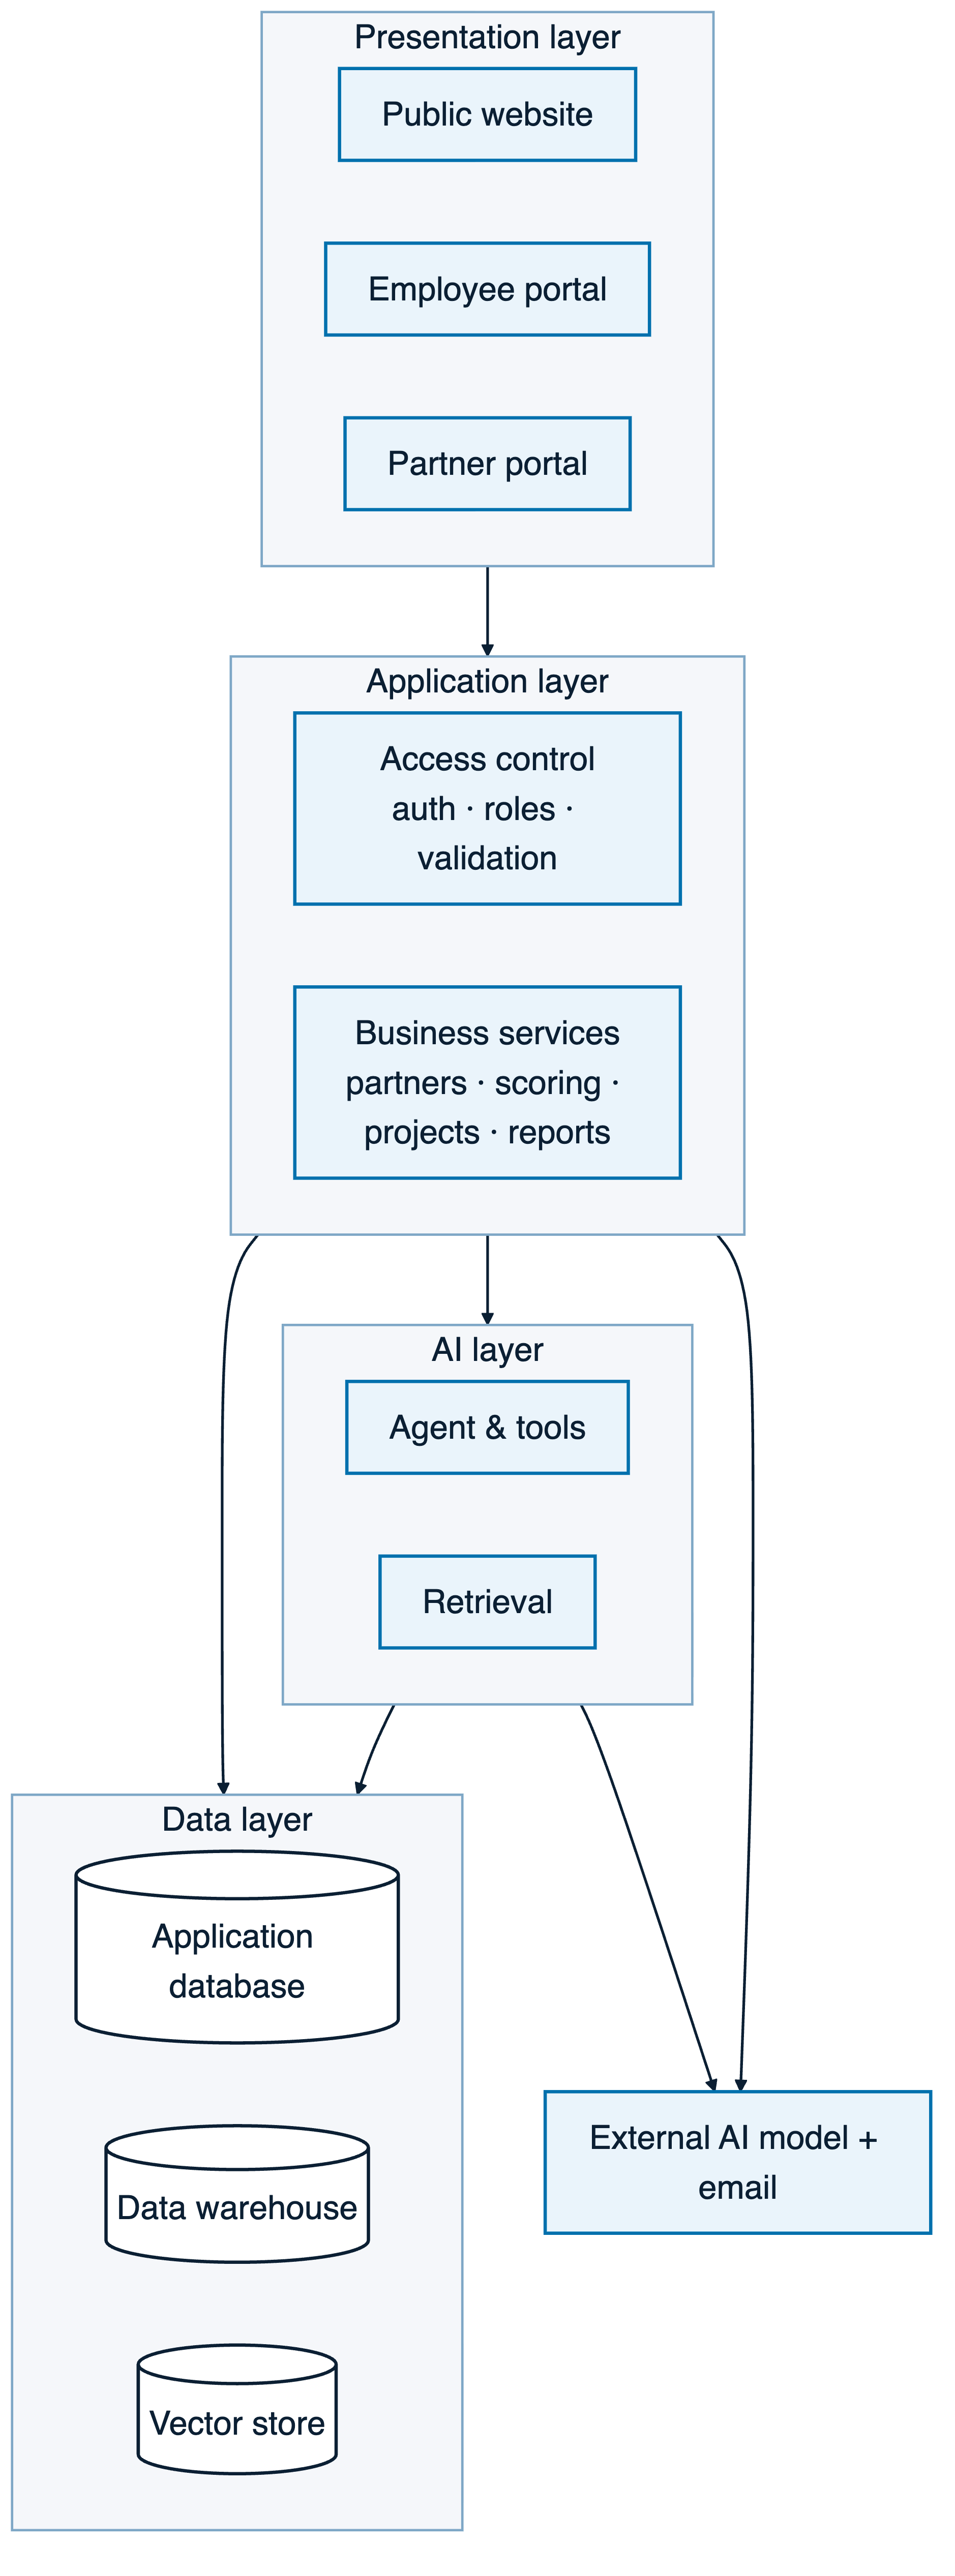
\includegraphics[width=0.78\linewidth,height=0.42\textheight,keepaspectratio]{figures/diagrams/architecture}
  \caption{Feature-driven monolith architecture of \projectname{}}
  \label{fig:feature-driven-architecture}
\end{figure}
The main responsibilities of each layer are:

\begin{itemize}
  \item \textbf{Access layer}: session extraction, password verification, token handling, and role-aware guards for protected requests;
  \item \textbf{Data layer}: the schema, migrations, the operational database client, and the data-warehouse configuration;
  \item \textbf{Service layer}: the business services for partners, scoring, projects, reporting, and shared server operations, which the business-intelligence engineer's module also consumes;
  \item \textbf{AI layer}: agent orchestration, typed tools, the retrieval pipeline, prompts, evaluations, and tool-result formatting.
\end{itemize}
\subsection{Layered Organization}
The application is a full-stack web app with server-rendered pages, thin request handlers, and a clear split between interface and business logic. Handlers receive input, check the current session, validate the payload, call the appropriate service, and return a structured response. Scoring, partner queries, project health, and report generation stay in the service layer so page code does not become the source of business truth.
\subsection{External Architecture}
From the outside, the system contains these blocks:

\begin{itemize}
  \item a browser client used by employees, partners, and public visitors;
  \item the \sourcecode{Next.js} application running the public website, employee portal, partner portal, API routes, and AI chat endpoint;
  \item the operational PostgreSQL application database storing users, partners, CRM data, projects, documents, reports, conversations, and audit traces;
  \item the PostgreSQL data-warehouse database storing BI-oriented analytical tables;
  \item external AI providers used for language generation and optional embeddings;
  \item an email provider used for platform notifications when configured.
\end{itemize}
The typical request flow is simple: the browser sends a request to a page or API route, the server authenticates it when required, validated input goes to a service, the service reads or writes through Drizzle ORM \netref{web:drizzle-docs}, PostgreSQL \netref{web:postgres-docs} persists the result, and the response returns as HTML, JSON, or a streamed AI message. External providers are used only for specialized capabilities.
\subsection{AI Subsystem Architecture}
The AI subsystem is an authenticated capability embedded in the same platform and governed by the same data-access rules as the rest of the product. Built around the AI SDK \netref{web:aisdk-docs}, typed tools, server-side orchestration, and RAG over curated business documents, it answers business questions, produces analyses, generates reports, searches documents, and calls platform tools without inventing facts.

\begin{figure}[htbp]
  \centering
  \dgram{ai-subsystem}
  \caption{Architecture of the agentic AI and RAG subsystem}
  \label{fig:ai-subsystem-architecture}
\end{figure}
The subsystem has five layers:

\begin{enumerate}
  \item \textbf{User interaction layer}: the agent workspace, suggestion prompts, conversation history, plan display, tool-result cards, charts, tables, and report cards.
  \item \textbf{Orchestration layer}: the chat route streams responses, manages tool calls, applies step and timeout limits, and formats assistant output.
  \item \textbf{Tool layer}: each tool has a typed input schema, a narrow business purpose, and access to server services rather than raw uncontrolled logic.
  \item \textbf{Retrieval layer}: document chunks and embeddings are stored close to business data; \sourcecode{pgvector} \netref{web:pgvector-docs} supports semantic retrieval, while metadata and ownership rules keep evidence scoped.
  \item \textbf{Governance layer}: tool traces, report records, source links, evaluation scripts, and structured failures make AI behavior reviewable.
\end{enumerate}
This design reduces the main risks of AI integration. The assistant stays a controlled interface over validated tools, explains its answers with sources, charts, and tables, and leaves authorization, validation, and persistence to the application.
\subsection{Two-Database Topology}
The platform uses two PostgreSQL databases: an operational application database and a data-warehouse database. This topology separates transactional collaboration data from analytical workloads while keeping the stack understandable and reproducible locally.

\begin{table}[H]
  \centering
  \caption{Two-database topology}
  \begin{tabularx}{\textwidth}{>{\bfseries\raggedright\arraybackslash}p{3.2cm}>{\raggedright\arraybackslash}p{3.8cm}X}
    \toprule
    Database & Main content & Purpose \\
    \midrule
    Application DB & Users, partners, contacts, offers, events, meetings, documents, projects, tasks, notifications, scores, AI threads, reports, audit records, and document chunks. & Supports operational screens, protected workflows, partner self-service, AI tools, RAG evidence, and transactional consistency. \\
    Data warehouse DB & Curated dimensional and fact-oriented tables for portfolio, category, partner, and project indicators. & Supports BI dashboards, aggregated metrics, analytical charts, and read-heavy reporting without overloading operational flows. \\
    \bottomrule
  \end{tabularx}
\end{table}
The application database is optimized for correctness and workflow execution, while the data warehouse is optimized for analysis and presentation. The separation also keeps demonstrations safer because BI views can evolve without weakening the operational schema.
\section{Technology Stack}
The selected stack supports a modern full-stack web application with strong typing, an efficient developer workflow, a consistent UI system, relational persistence, analytics, and AI integration.

\begin{table}[H]
  \centering
  \caption{Technology stack}
  \begin{tabularx}{\textwidth}{>{\bfseries\raggedright\arraybackslash}p{3.2cm}
                               >{\raggedright\arraybackslash}p{4cm}
                               >{\raggedright\arraybackslash}X}
    \toprule
    Area & Technology & Role in the project \\
    \midrule
    Framework & \sourcecode{Next.js} App Router \netref{web:nextjs-docs} & Full-stack routing, layouts, server components, API routes, streaming endpoints, loading states, and error boundaries. \\
    UI library & \sourcecode{React} \netref{web:react-docs} & Component-based interface composition for public pages, employee dashboards, partner portal, and AI workspace. \\
    Language & \sourcecode{TypeScript} \netref{web:typescript-docs} & Static typing for route contracts, component props, server services, AI tool schemas, and database-facing logic. \\
    Runtime and scripts & \sourcecode{Bun} \netref{web:bun-docs} & Dependency management, local development, build scripts, database scripts, seed routines, and evaluation commands. \\
    Styling & \sourcecode{Tailwind CSS} \netref{web:tailwind-docs} & Token-driven responsive styling, spacing discipline, light and dark modes, and rapid UI composition. \\
    UI primitives & \sourcecode{shadcn/ui} \netref{web:shadcn-docs} & Accessible component foundations for buttons, forms, dialogs, tables, alerts, and layout primitives. \\
    ORM & \sourcecode{Drizzle ORM} \netref{web:drizzle-docs} & Type-safe SQL modeling, schema centralization, migrations, and database queries. \\
    Database & \sourcecode{PostgreSQL} \netref{web:postgres-docs} & Operational persistence and analytical storage through the application database and data warehouse. \\
    Vector search & \sourcecode{pgvector} \netref{web:pgvector-docs} & Storage and similarity search for document embeddings used by RAG. \\
    AI orchestration & \sourcecode{AI SDK} \netref{web:aisdk-docs} & Streaming chat responses, tool calls, structured outputs, and agentic workflow integration. \\
    Data warehouse backend & \sourcecode{Python} \& \sourcecode{FastAPI} & External backend powering the data warehouse analytics pipeline; used in a companion data-engineering service that feeds the BI layer. This component is part of the broader project delivery but not the primary product responsibility. \\
  \end{tabularx}
\end{table}
Together, these choices produce an architecture that is ambitious enough for an AI-enhanced enterprise platform but still realistic for a final-year project. The same stack supports user-facing pages, server-side business rules, database access, BI, document retrieval, and AI-assisted reporting without multiplying runtime models.
\section*{Conclusion}
\addcontentsline{toc}{section}{Conclusion}
This chapter established the planning and architecture foundation of \projectname{}. The actor analysis clarified the responsibilities of Admin, Manager, Commercial, Analyst, HR, and Partner users. The functional and non-functional requirements defined what the platform must do and how reliably it must behave. The Product Backlog and six-sprint plan turned the scope into an incremental roadmap across the internship. Architecturally, the project is a feature-driven monolith with presentation, application, AI, and data layers, built with strict \sourcecode{TypeScript}, reusable components, thin request handlers, and server services. The external architecture keeps the operational core inside the application while using external providers only for specialized AI and email capabilities. The AI subsystem is governed, tool-based, and source-grounded. The two-database topology separates operational persistence from analytical workloads and gives the platform a solid foundation for the implementation chapters that follow.
